\section{Тестирование работоспособности программного средства}

\subsection{Тестирование функции построения карты}
Тестирование функции построения карты:
Изначально тестирование ПО производилось в симуляции на ПК. В качестве симулятора была выбрана среда WeBots
из-за лёгкости интеграции языка программирования Rust.


\begin{figure}[H]
\centering
	\fbox{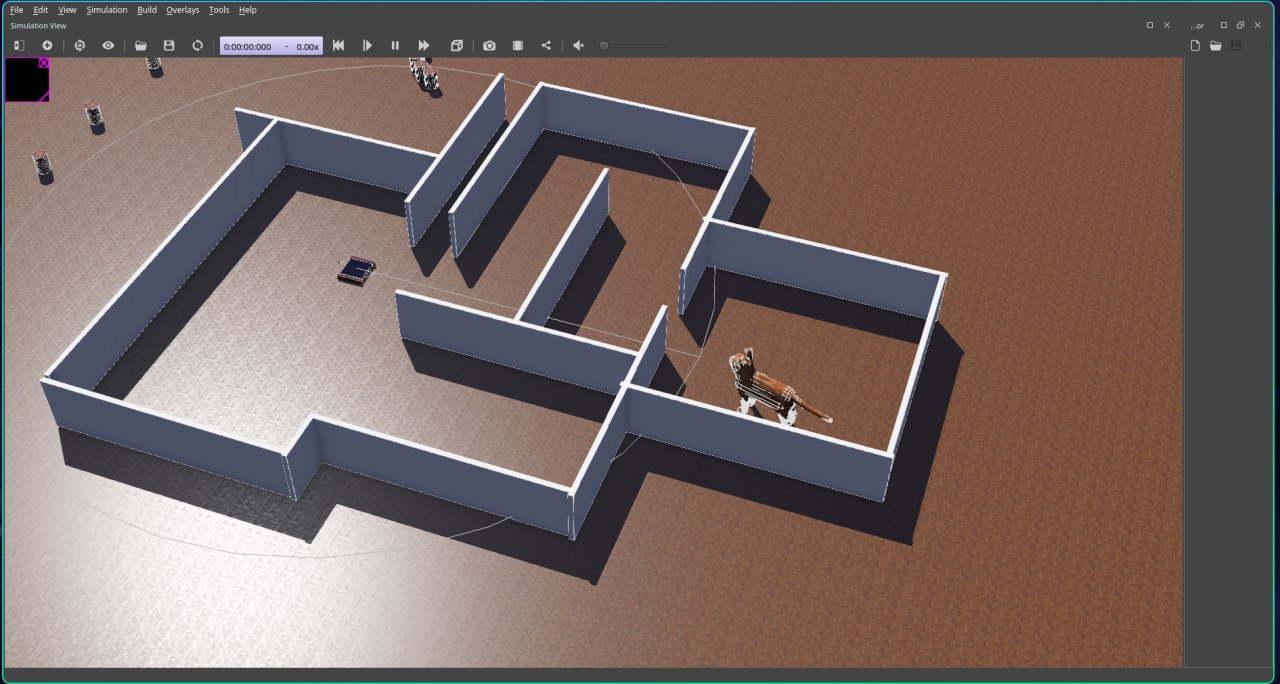
\includegraphics[width=15cm]{webots_screenshot.jpg}}
\caption{Среда симуляции WeBots}
\label{fig:components}
\end{figure}


\subsection{Тестирование базовой навигации}
Цель: убедиться, что робот может перемещаться из точки A в точку B по прямой линии без препятствий. \\ {Метод}: В симуляторе Webots была создана простая среда без объектов, и роботу была задана задача достичь целевой точки. \\
{Результат}: Робот успешно достиг целевой точки, продемонстрировав корректную работу датчиков и базового алгоритма движения.

\subsection{Тестирование при наличии статических препятствий}
Цель: Проверить, как алгоритм строит маршрут, обходя неподвижные объекты. \\
{Метод}: В среде были размещены стены и коробки, и роботу была задана задача их обойти. \\
{Результат}: Алгоритм точно обнаружил препятствия и спланировал безопасный путь, избегая столкновений.

\subsection{Тестирование при наличии динамических препятствий}
Цель: Оценить адаптацию алгоритма к движущимся объектам. \\
Метод: В симуляцию были добавлены движущиеся объекты, и была проверена реакция робота. \\
Результат: Робот успешно избегал столкновений с движущимися объектами, демонстрируя быструю реакцию на изменения.

\subsection{Тестирование в сложных средах}
Цель: Проверить работу алгоритма в запутанных пространствах. \\
Метод: Была создана карта с множеством поворотов и тупиков. \\
Результат: Алгоритм нашел оптимальный путь и избежал зацикливания, что подтверждает его эффективность в сложных условиях.

\subsection{Тестирование при сбоях датчиков}
Цель: Оценить устойчивость алгоритма к неточным данным. \\
Метод: В симуляции были смоделированы отказы датчиков и добавлен шум к их показаниям. \\
Результат: Алгоритм продолжил выполнение задачи, справившись с ошибками и неточностями данных.

\subsection{Тестирование локализации}
{Цель}: Проверить точность определения местоположения робота на карте. \\
{Метод}: Были использованы алгоритмы SLAM для построения карты и локализации. \\
{Результат}: Карта была построена с высокой точностью, и робот успешно корректировал свою позицию при ошибках.

Все проведенные тесты были успешно пройдены, что подтверждает высокую эффективность, надежность и адаптивность разработанного алгоритма построения карты и нахождения пути. Результаты тестирования позволяют рекомендовать данный алгоритм для использования в реальных условиях.
